\documentclass[]{article}   % list options between brackets
\usepackage{float}              % list packages between braces
\usepackage[english]{babel}
\usepackage{graphicx}

\begin{document}

\title{Mario: A Machine Learning Classification Approach}   % type title between braces

\author{Erek Speed and Nick Villalva}         % type author(s) between braces
\date{December 6, 2011}    % type date between braces
\maketitle

\begin{abstract}
 The purpose of this project was to construct a 
\end{abstract}

\section{Introduction}     % section 1
This project is a departure from the common data sets of the machine learning world. The authors have eschewed corpi and proteins in lew of something a bit closer to their hearts.  To this end, we've repurposed the classification powers of the machine learning world for use with a classic platforming game from our youth, Super Mario Brothers(Mario).  Despite the levity of the topic, the discussion of the algorithms is just as reasonable as the common problems of the field.  Indeed, if we consider the Mario world a rough approximation of our own then it's easy to see the relevance of of studying a simpler version of what some might consider the holy grail of artificial intelligence: human level interaction with arbitrary environments.
\newline\newline
To that end, this end the work here explores treating world interaction as a classification problem.  Specfically, we want to classify every possible state of the world as a particular action. Taking such an action would lead to a new state and a new action.  By continuing in this fashion a agent explores the world in the manner it was trained.
\newline\newline
With such a vision, the present work describes and evaluates the application of popular machine learning algorithms to our lofty task.  We start with a discussion of the of previous work in the mario AI area.  In general, no standing body of data exists for Mario domain.  To overcome this obstacle we developed a system for a generating a dataset cooresponding to optimal actiosn in response to the current environment.  A description of this process and various attempted optimizations appears in \ref{sec:datagen}.  With data in hand, the authors attempt to create a Mario agent by applying popular machine learning algorithms to said data.  Each classifier is described in turn in section \ref{sec:class}.  \ref{sec:results} evaluates the previously described classifiers using common performance metrics as well as actual performance on unknown Mario levels.  We end with a discussion of future work and a conclusion.

\subsection{Division of Work}

\section{Previous Work}
\label{sec:prevwork}
The present work is the first to attemp to solve Mario as a classification problem.  That said, in recent years there has been a surge of attempts to develop Mario playing Agents.  The interest started with a MarioAI contest in 2009 which solicited all computer agent solutions to the Mario problem \cite{2}.  Interestingly, the report from said contest was dominated by handcoded such as A* \cite{3}.  In fact, due to the ability to reverse engineer the simulation engine the problem was reduced to a planning problem and easily solved.  A scattering of learning algorithms involving neural networks and genetic algorithms were submited but performed poorly.  Later, learning algorithms were given their own category in which they only had to learn a single level. With such a constraint, learning algorithms were able to reach near optimal performance \cite{me}. In contrast, we reject the notion that Mario is only solvable with complete prior knowledge of the the world.  We also acknowledge the vastness of the problem space and the failures of past learning problems getting lost in its many plateaus.  By creating an agent which trains on data generated from an expert player we greatly shink the problem space while maintaining some amount of generality.  



\section{Data Generation}     % section 2.1
\label{sec:datagen}
It is a nice metephor to imagine a untrained novice classifier viewing instance after instance of data derived from studying an expert agent.  In order to make such a thought reality, one not only needs a source of expert data to mine but also needs to massage it into a convenient format for current machine learning problem.  The following subsections will describe the initial state of the data, the conversion to a more general form, and finally performance optimizations.
\subsection{MarioAI Benchmark}
The MarioAI Benchmark \cite{mariobenchmark} was developed in order to facilitate the developing and testing of AI agents.  It placed the original software in a wrapper which the creators felt would allow easier creation of all kinds of agents.  For instance, while the various locations of objects in the world are represented as continuous variables, but the benchmark wraps the low level data in a representation which discretizes the data into a convenient grid like format [figure].  Each cell of the grid contains a integer relating to its contents.  Furthermore, the agent has access to public information outside the grid, including whether it is alive or dead, on the ground, and it's status(size, powers).  Given this information, the agent is expected to return an action which coressponds to the buttons that might be pressed in the original game.  In order to gather data, we use a script which records the state and action pairs generated as a trained agent \cite{me} plays expertly.  By modifying the parameters of generated environments, millions of unique data points can be generated in minutes.
\subsection{Data Conversion}
Obviously, the representation has an obvious analog to common formats used in machine learning.  If we consider each grid space as feature then we can use it directly as a feature vector into a learning algorithm.  Furthermore, we can simply append the extra public information to the end to complete the vector.  Unfortunately, while this would be a valid input to most algorithms, the data is certainly not optimal.

The first problem is that the values chosen to represnt the contents of each feature are seemingly random.  The scattering of the values are such that it the features appear continous upon first glance.  Unfortunately, upon further inspection it becomes obvious that the specific values a feature may take have no deeper meaning and would lead to poor results in many algorithms requiring placing the vectors in some measured space.  To solve this problem, we identified the possible values and grouped them into 13 cateogories.  For consistent weighting of every discrete value, we also expanded each feature into 13 binary levels.  At this point, the data is ready to be exported for classifier consumption.  Following the example of current software packages, we represented the vectors using a sparse indictor variable.  Using the default settings of the benchmark (19x19 grid) and including a few of the most important state flags we end up with a feature vector in 4697 dimensions.

\subsection{Optimizations}
Given the data described so far, it's possible to apply common algorithms and get valid results.  Unfortunately, for many software packages such a large data set in this many dimensions is simply intractable.  For example, $k$nn scales teribly with large numbers of dimensions.  In order to take advantage of such classifiers we applied various feature reduction strategies.
\newline\newline
The primary method we used was a greedy forward selection algorithm which considered each attribute compared with the class distribution.  The software we used allowed specifying the distance metric for comparing the attribute vector with the class vector, but with our data such methods differed little.  Examples of metrics include Euclidean distance, the Pearson coefficient, and symmetrical uncertainty.  Unfortunately, this construction doesn't reduce redundancy amongst the features which leads to the smaller feature subsets being with correalated albeit relevant features.  As an extreme example, the top two features included a state flag "isMarioOnGround" and a grid attribute "is grid space below Mario solid ground."  Regardless of shortcomings, creating datasets with 1,5, and 10 percent features allowed tractable classification.
\newline\newline
The second feature selection optimization is simply one of reasoning.  We realized that the most important features are the ones closest to the Mario agent.  With this in mind, we produced data sets that reduced the grid size from 19x19 to 5x5.  This not only allowed algorithms to complete training faster, but it also allowed them to focus on the most important features.
\newline\newline
The final optimization left the feature vector size alone but instead dealt with the problem of noise.  The most advanced Mario agents will sometimes make erratic actions in the interest of exploring the worlds and finding hidden secrets.  The subset of possible environments used for the present work, however, requried very little exploration.  Upon such realiziation, the parameters of observed expert were changed such that almost all erratic behavior was removed.  This allowed nosie sensitive algorithms like SVM to work better.

\section{Classifiers}
\subsection{Software}
\subsubsection{Libraries}
We considered several libraries for this project and ultimately settled on Java ML \cite{javaml}. Our main 
requirements were that it support the various classifiers we wished to use, have an implementation of feature 
selection, and be capable of interfacing with the Mario Benchmarking \cite{mariobenchmark} software. The 
Mario software was obtained from the MarioAI competition and is written in Java. It allows for the use of 
players that implement an Agent interface to take in data about the world and push buttons on the controller 
to move Mario as it sees fit. We looked at using weka \cite{weka}, Java ML \cite{javaml}, scikit-learn 
\cite{scikit}, and libsvm \cite{libsvm}. 

Weka is a relatively full featured library written in java, and as such was one of the most attractive libraries 
available. It is well used and contains all of the types of classifiers we hoped to use. The major drawback 
surrounding the use of weka was the data format it required. Programatically it was rather complicated to setup 
data on the fly, and translating the datafiles we had already created into the proper format was a taxing proposition. 

Scikit, written in python, was considered due to the ease of data manipulation in python and the fact that both 
of us were comfortable with the language. The major drawback of this is that we would have to find a way to 
export all of our classifiers and import them into the java based Mario Benchmarking software. The libsvm 
integration with scikit was very appealing and was one of the major reasons we considered it.

Libsvm was a great choice because its widespread use and its proficient handling of various multiclass support 
vector machines. What made us shy away from direct use of libsvm was that all three other libraries had wrappers 
for libsvm that would allow us to reap its benefits from within a single library that contained all of our classifiers.

We ultimately chose Java ML due to its simple data interface, native java compatibility, and the fact that it 
wrapped both Weka and libsvm functionality. This enabled us to use libsvm for our support vector classifiers, 
wrapped Weka classifiers for random forests, na\"{i}ve Bayes, KNN and REP trees, and forward and backwards feature 
selection. 

\subsection{KNN}
\subsubsection{Reasons for selection and expectations}
We chose to include k nearest neighbors as one of our algorithms because we thought that the large search space 
would help it identify similarities between attributes in our dataset. Hopes were high for the reduced feature 
sets as they should only be looking at the attributes that have an impact on the action to be taken for a given 
board configuration.  We expected KNN to train slowly and respond slowly, making it less than ideal for actual play. 
However, the simplicity of the algorithm would give us a good baseline for what is possible.

\subsubsection{Parameter selection}
KNN had very few parameters to select – the number, $k$, of neighbors to look at and the distance measure that would 
be used to find the nearest neighbors. First, due to the scarcity of data for some of our classes, we chose to 
experiment with $k$ from one to five. We then selected a few distance measures to test – Euclidian, symmetric uncertainty 
and Jaccard indexing. We then ran a grid search using five-fold cross validation to determine the best set. The metrics 
we measured to compare the success of classifiers with one another were accuracy, precision, f1 and recall. 


\subsection{Na\"{i}ve Bayes}
\subsubsection{Reason for selection and expectation}
Na\"{i}ve Bayes was an attractive classifier to use since it allowed for priors, allowed us to view a probability 
distribution on optimal actions, and yielded classifications relatively quickly. We expected it to perform decently 
with the full ensemble of data, but really shine with a reduced dataset that hopefully proved to have a better 
signal to noise ratio. 

\subsubsection{Parameter selection}
The wrapped implementation of na\"{i}ve Bayes provided by Java ML required very few parameters. We were given the 
option of using a Laplace correction as a prior and the use of logarithmic results. As our dataset was sparse, we 
were appreciative of the ability to make the classifier aware of this in order to improve performance. Due to the 
very limited number of parameters, our grid search for optimal parameters focused on whether or not to include a 
Laplace correction and the size of dataset on which the classifier was trained. 

\subsection{REP Trees}
\subsubsection{Reason for selection and expectation}
REP (Reduced Error Pruning) trees, while not specifically covered in class, were used as a representative of the 
various tree classsification methods. This algorithm builds a decision/regression tree and internally splits the 
dataset into folds in order to perform reduced error pruning. The key motivation for including REP trees in our 
ensemble of classifiers was to have a tree that actively prunes itself as they are purported to be especially good 
at classifying categorical data. We expected the tree to take longer to train than KNN or na\"{i}ve Bayes, but to 
respond to requests quickly.

\subsubsection{Parameter selection}
The REP tree algorithm we utilized required a few parameters -- the minimum number of records per leaf, the number 
of folds for pruning, and the maximum depth. Due to the size and imbalance of our data, we decided to retain most 
of the default settings of three folds, no maximum depth and two instances per leaf. Our experimentation with REP 
trees focused on the amount of data provided for training and its impact on the accuracy of the classifier.

\section{Results}
\subsection{Metrics}
In evaluating our methods we decided to use a combination of accuracy, precision, recall and f1 characteristics to 
evaluate our cross validation results for KNN, SVM and na\"{i}ve Bayes. As the tree algorithms do not measure these
statistics, we used root mean squared error as our metric.

Similarly, a metric was needed to compare results from runs through the Mario 
Benchmark. The metrics picked for that were a combination of a weighted fitness score that the benchmarking program 
calculated and a scalar progress count that represented how far through the level the classifier controlled Mario was 
able to get. The following analyses are based on these metrics.

\subsection{KNN}
\subsubsection{Cross Validation}
Running five-fold cross validation on KNN revealed interesting results. Cross validation revealed that 3 was the optimal
choice for $k$. The first thing we noticed was with respect to the distance measures -- Euclidean distance was worse than
the Jaccard index for out data. In cross validation, the best results achieved with Euclidean distance were precision of 0.645,
accuracy of .851, recall of .0327 and F1 measure of .0472. Due to many classes not being chosen, precision could not be averaged
across the datasets for a few configurations. The results are below.

\begin{table}[h!]
	\begin{center}
		\caption{Cross validation results for KNN}
		\begin{tabular}{l | l || l | l | l | l }
		Data Size & Feature Reduction & Precision & Accuracy & Recall & F1 Measure \\
		\hline
		20K & 99\% & 0.915 & 0.989 & 0.0597 & 0.0625 \\
		20K & 95\% & 0.920 & 0.990 & 0.0599 & 0.0625 \\
		20K & 90\% & 0.917 & 0.989 & 0.0598 & 0.0625 \\
		2.5K & 5x5 & 0.837 & 0.988 & 0.101 & 0.0957 \\
		2.5K & 5x5 & 0.882 & 0.991 & 0.101 & 0.0956 \\
		\hline
		\end{tabular}
	\end{center}
\end{table}

\subsubsection{Mario Benchmark}
As expected, the KNN algorithm was incredibly slow to respond to move requests. Additionally, as eluded to by the invalid precision
results on some of the cross validation, the majority of responses consisted of holding down the forward and jump buttons continually
in a manner that prevented Mario from doing more than one jump per level. As such, the KNN classifiers never finished a level. The best
performance of the classifier was on the simplest level on the lowest difficulty with a weighted fitness of 1488. It was able to make its
way through 26.9\% of the level.

\subsection{SVM}
\subsubsection{Cross Validation}
Cross validation for our support vector machines was done with two-fold validation, as the size of our datasets made 
it very costly time-wise to perform more than two-fold validation. A grid search was done for parameters using both linear
and RBF kernels. The best linear svm was produced by $C = .01$ with a score of $0.9842$, and the best RBF svm was produced by
$\gamma = .5$ and $C = 10$ with a score of $0.6999$.

\subsubsection{Mario Benchmark}
The performance of our trained SVMs on the benchmark was rather interesting. With data reduction of 99\% (the 1\% dataset), the support
vector machine was incapable of learning to pass the simplest level which requires running forward and jumping. It consistently
collided with a ledge and got stuck until time ran out. With data reductions of 95\% or less, the SVM was capable of learning to
run forward and jump repeatedly, allowing it to pass the simplest levels. The RBF svm identified by cross validation finished every
level that contained no gaps, enemies or blocks, and was capable of finishing the easiest level that included gaps. The linear svm
identified by cross validation was unable to complete a level in spite of its superior cross validation results. Behaviorally, it
never let go of the jump button and therefor Mario was unable to jump after his first hop.

\subsection{Na\"{i}ve Bayes}
\subsubsection{Cross Validation}
Cross validation of the various na\"{i}ve Bayes classifiers alerted us that it would not be a very good player. For an example of the
performance as evaluated by five-fold cross validation, the results for 20,000 datapoints with various levels of feature reduction are
shown below.

\begin{table}[h!]
	\begin{center}
		\caption{Cross validation results for Na\"{i}ve Bayes}
		\begin{tabular}{l | l || l | l | l | l }
		\hline
		Data Size & Feature Reduction & Precision & Accuracy & Recall & F1 Measure \\
		\hline
		20K & 99\% & 0.133 & 0.967 & 0.0751 & 0.0973 \\
		20K & 95\% & 0.077 & 0.931 & 0.0565 & 0.0935 \\
		20K & 90\% & 0.082 & 0.943 & 0.0617 & 0.0864 \\
		\hline
		\end{tabular}
	\end{center}
\end{table}

\subsubsection{Mario Benchmark}
Much like the linear svm, none of the nai\"{i}ve Bayes classifiers were able to complete a level on the benchmark. The highest fitness
value found was shared between four different parameter settings. Classifiers trained with the 5x5 dataset with both 5000 and 10,000
datapoints were capable of scoring a 1913 on the easiest level. Likewise, Classifiers trained on the 5\% and 1\% datasets with 20,000
datapoints achieved the same score.

This alludes to an interesting threshold difference between the reduced datasets and the 5x5 grid data. Reduced datasets required four
times as many datapoints to achieve the same level of success as the 5x5 grid with a Bayesian classifier. Intuitively this does not make sense,
as the length of the feature vectors in the 1\% and 5x5 datasets were about the same. 

\subsection{REP Trees}
\subsubsection{Cross Validation}
As previously mentioned, cross validation of REP trees was performed by measuring the root mean squared error. Using the various levels of feature
reduction and changing the number of folds used by the algorithm did not change this metric. This makes sense because it should choose the optimal
features to look at and use as few of them as possible. The root mean squared error of our REP trees was $0.0353$.

\subsubsection{Mario Benchmark}
REP trees were one of the few classifiers to successfully complete the clear levels with ledges consistently while showing the lowest threshold for
datapoints required to reach optimality. 

\begin{table}[h!]
	\begin{center}
		\caption{REP tree classifiers capable of scoring the highest score}
		\begin{tabular}{l | l || l  }
		\hline
		Data Size & Feature Reduction & Score \\
		\hline
		500 & 5x5 & 6568 \\
		500 & 95\% & 6568 \\
		500 & 90\% & 6568 \\
		\hline
		\end{tabular}
	\end{center}
\end{table}

Also of note is that with 99\% feature reduction, the REP trees were unable to complete the level. This suggests that a key feature for learning to 
rest between jumps is discarded with the move from 95\% to 99\%.

\subsection{Random Forests}
\subsubsection{Cross Validation}

\subsubsection{Mario Benchmark}

\subsection{Overall}

The overall performance of the classifiers is best communicated through graphical representations of the weighted fitness score of the best classifier
of each category graphed against each other. It is very interesting to note the similarities in performance between the REP tree algorithm and the SVM,
whose scores are nearly identical for every configuration. This leads us to believe that both algorithms found the ideal means of separating our data.


As can be seen in Figure 1, REP tree and SVM are indistinguishable and highly successful with simple levels devoid of gaps, blocks or enemies. Random
forests, KNN and naive Bayes all struggle, with the best and most inconsistent of them being the random forest.
\begin{figure}[H]
\centering
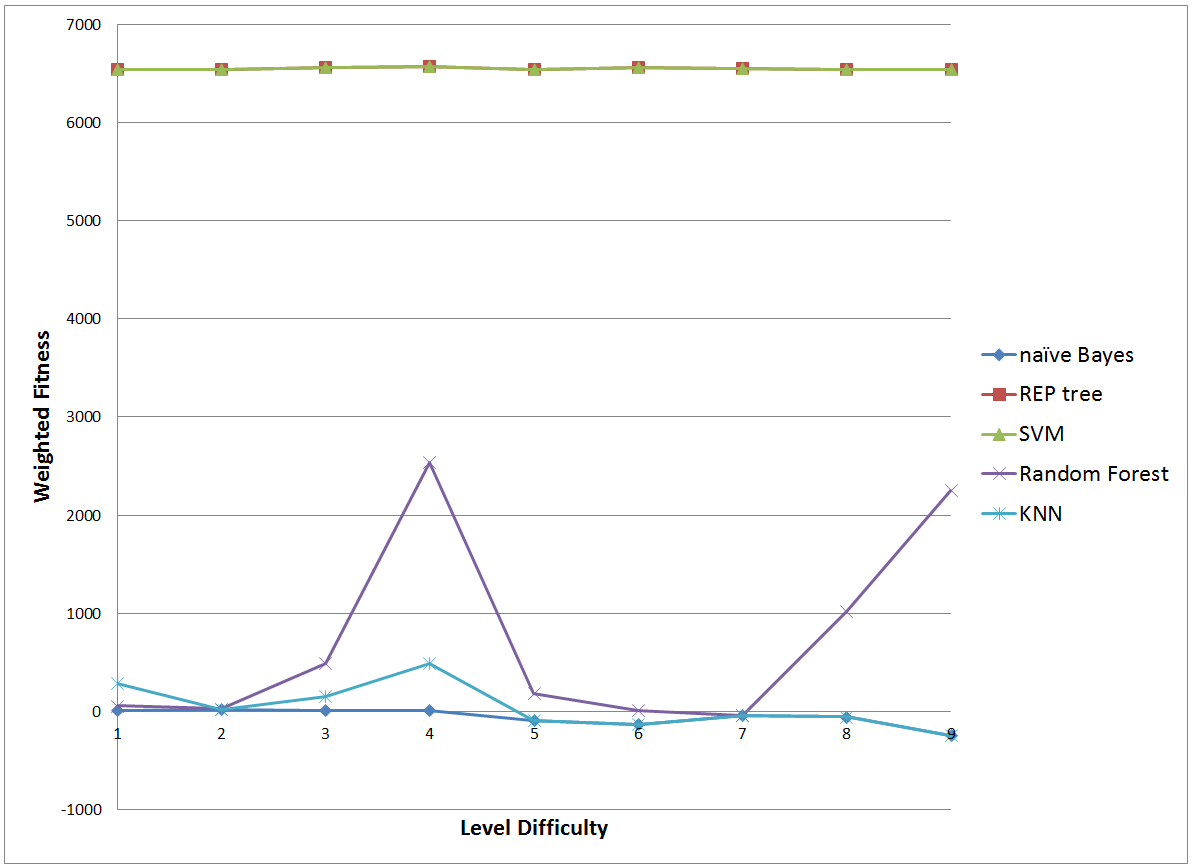
\includegraphics[width=90mm]{basic.png}
\caption{Graph of performance on basic levels by classifier}
\end{figure}

For levels including gaps (Figure 2), REP tree and SVM succeed at the easiest level and remain the most successfull as difficulty increases. Random forest is once again
very erratic in its performance while KNN and naive Bayes fluctuate but remain the worst performers.
\begin{figure}[H]
\centering
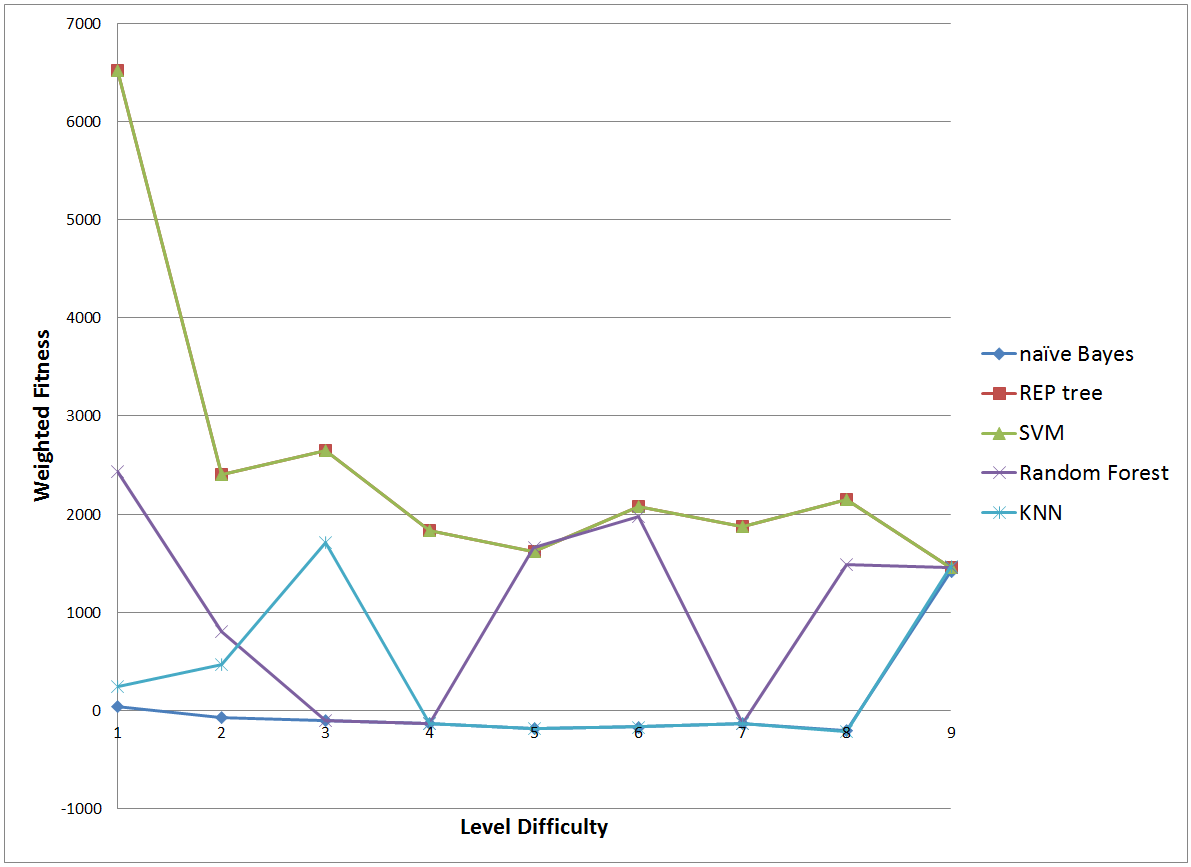
\includegraphics[width=90mm]{gaps.png}
\caption{Graph of performance on levels with gaps by classifier}
\end{figure}

When enemies are added to the levels, none of the classifiers can successfully navigate a level. As can be seen in Figure 3, the classifiers converge
to a point for the highest difficulty and the general general trend is a decrease in score as difficulty increases. This suggests that the presence of enemies
is an equalizer between the usual highly successful REP tree and SVM and the rest of the classifiers.
\begin{figure}[H]
\centering
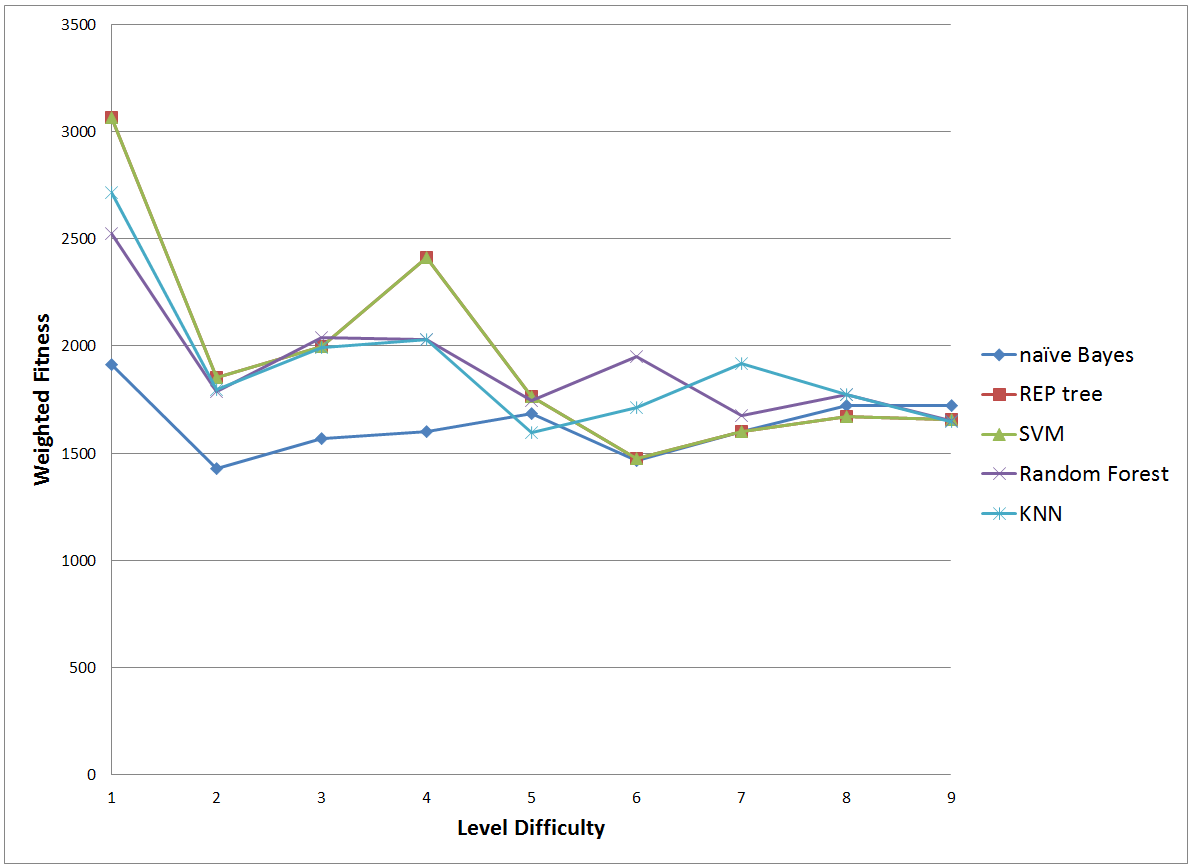
\includegraphics[width=90mm]{enemies.png}
\caption{Graph of performance on levels with enemies by classifier}
\end{figure}

When both enemies and blocks are present, all classifiers have an eratic performance. The REP tree and SVM pair are still the best performing overall. Random
forest shows a bit of promise for the middle difficulties, even doing better than REP trees on level six. Overall, performance with enemies and blocks is unreliable
and a bit random as can be seen in Figure 4.
\begin{figure}[H]
\centering
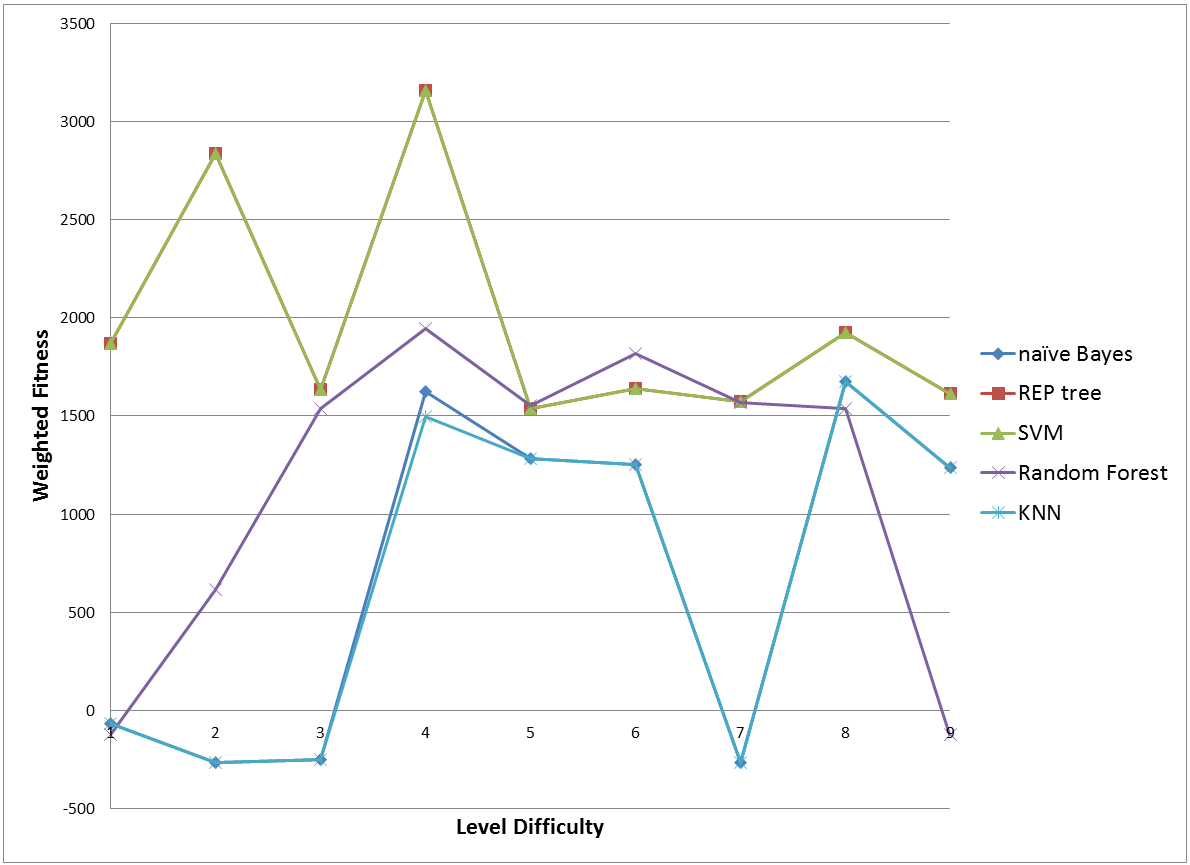
\includegraphics[width=90mm]{enemiesblocks.png}
\caption{Graph of performance on levels with enemies and blocks by classifier}
\end{figure}

The final situation the classifiers were tested on was levels with enemies, blocks and gaps present. As can be seen in Figure 5, the classifiers finally become 
more stratified than in the previous four examples. SVM and REP tree are still identical and the best overall with a sharp decline for difficulties greater than 1, but 
random forests now does consistently better than naive Bayes or KNN. As this level is the most like levels that would appear in the real Mario games, this is the most
interesting one to see, and really signifies the difficulty of a learning agent successfully navigating a level.
\begin{figure}[H]
\centering
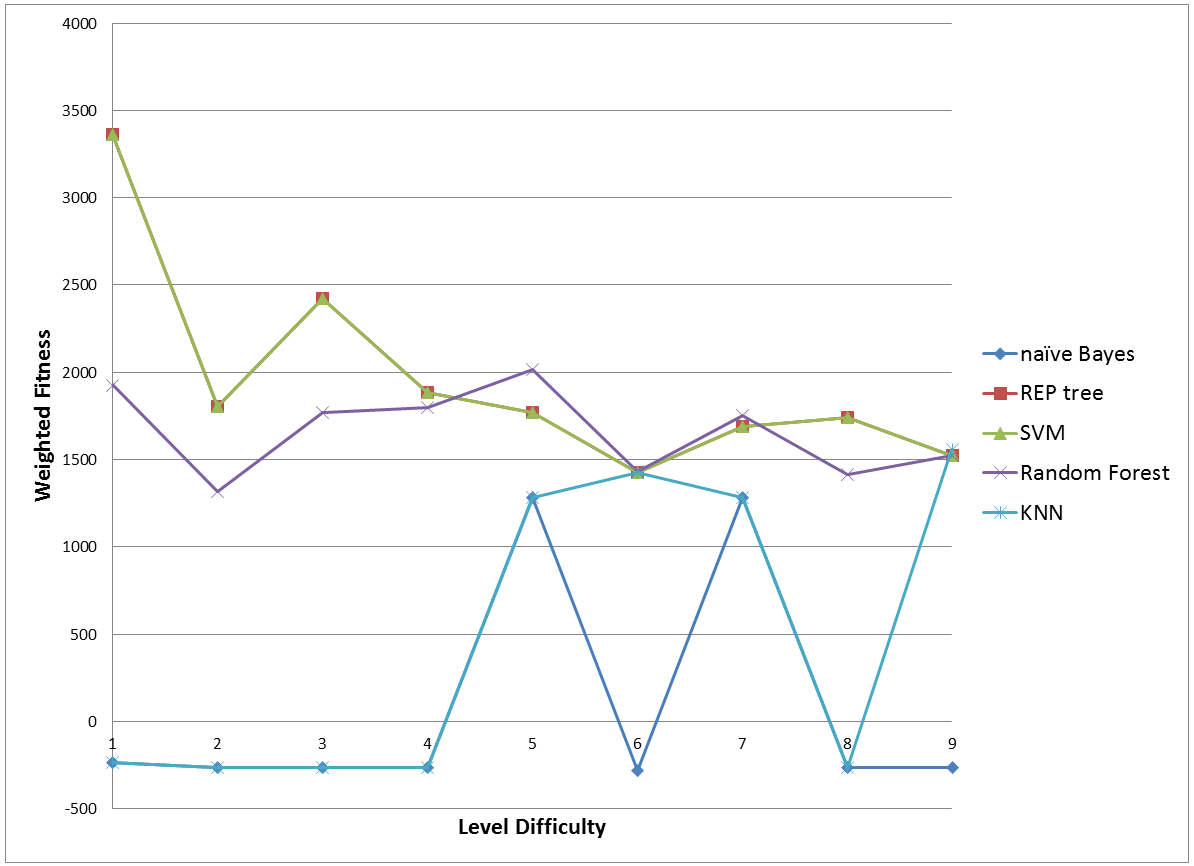
\includegraphics[width=90mm]{enemiesblocksgaps.png}
\caption{Graph of performance on levels with enemies, blocks and gaps by classifier}
\end{figure}

\section{Future Work}

Having examined the source code of the Java ML library that we used, the implementation of some algorithms was not entirely correct. Unfortunately we realized this with too
little time to switch to a new library and re-run all of our tests, so the first thing we would do if we were to continue this avenue of exploration would be to validate
these results using a second library, such as Weka.

Further improvements could be attempted by implementing adjustments for the sampling imbalance of our data, such as the SMOTE algorithm.

Priors could be better enforced by weighting the value of data gathered from nearest Mario higher than that gathered from across the screen. Various examples of this would be
starting with the weight of Mario's square being 100 and decreasing with weight as a function inversely proportional to the distance from Mario. We attempted to do this in a
small fashion with the 5x5 dataset, though it would be interesting to see additional approaches.

\section{Conclusion}

Through this exercise, we have determined that at this time, the classifiers we tested are not suitable for playing a level of Mario that contains gaps, blocks or enemies.
At their best, they are capable of immitating a basic forward jumping agent that continually jumps as it runs across the level. At their worst, classifiers run into walls for
minutes on end or walk back and forth through the same two squares. Additional work must be done for classifiers to stand a chance against Mario agents programmed to use
reinforcement learning, genetic algorithms or modified A*.


\begin{thebibliography}{9}
  % type bibliography here
  \bibitem{javaml}
  Abeel, T.; de Peer, Y. V. \& Saeys, Y. Java-ML: A Machine Learning Library, Journal of Machine Learning Research, 2009, 10, 931-934
  \bibitem{mariobenchmark}
  Diego Perez, Miguel Nicolau, Michael O'Neill, Anthony Brabazon: Evolving Behaviour Trees for the Mario AI Competition Using Grammatical Evolution. EvoApplications(1), 2011: 123-132 http://www.marioai.org/
  \bibitem{weka}
  Mark Hall, Eibe Frank, Geoffrey Holmes, Bernhard Pfahringer, Peter Reutemann, Ian H. Witten; The WEKA Data Mining Software: An Update; SIGKDD Explorations, 2009, Volume 11, Issue 1.
  \bibitem{scikit}
  Pedregosa, F.; Varoquaux, G. et. al. Scikit-learn: Machine Learning in Python, Journal of Machine Learning Research, 2011, 12, 2825-2830
  \bibitem{libsvm}
  Chang, Chih-Chung and Lin, Chih-Jen, {LIBSVM}: A library for support vector machines, ACM Transactions on Intelligent Systems and Technology, 2011, Volume 2, Issue 3, 27:1-27:27
\end{thebibliography}

\end{document}
